% 3. Protokoll

% Variables
\def\skalierung{0.65}

\chapter{Messprotokoll}
\label{chap:protokoll}

\section{Probenpräparation}
\label{sec:prep}

\subsection{Substratherstellung}
\label{sub:substrat}
Als Substrat werden Glasplätchen verwendet die in passender Länge (~\SI{2,5}{\centi\metre}) und Breite (~ß\SI{1,5}{\centi\metre}) zugeschnitten, welche dann wiederum mit dem Schema \textit{GruppennummerSubstratnummer} (z.Bsp. 13 (Substrat 3) und 111 (Substrat 11)).

\subsection{Stammlösung}
\label{sub:stamm}
Als Stammlösung wird Polystyrol (PS) und Chlorbenzol (CB) verwendet. Diese werden im dem Fläschen \enquote{\textit{PS-CB; \SI{300}{\milli\gram\per\milli\litre}; Gruppe 1}} angerührt. Dabei erhalten wir \SI{297,92}{\milli\gram} PS, was zur Folge hat, dass \SI{0,9931}{\milli\litre} CB zugegeben werden muss, um die gewünschte Konzentration von \SI{300}{\milli\gram\per\milli\litre} zu erhalten.

\subsection{Verdünnung}
\label{sub:verduennung}

Um aus der angesetzte Lösung aus Kapitel \ref{sub:stamm} die gewünschten Konzentration von \SI{1}{\milli\gram\per\milli\litre}, \SI{25}{\milli\gram\per\milli\litre}, \SI{50}{\milli\gram\per\milli\litre}, \SI{100}{\milli\gram\per\milli\litre}, \SI{150}{\milli\gram\per\milli\litre}, \SI{200}{\milli\gram\per\milli\litre} und \SI{250}{\milli\gram\per\milli\litre} zu erhalten, werden folgende Formeln verwendet:
\begin{gather}
	V_0 = V_S + V_{CB}\\
	\boxed{V_{CB} = V_0 \cdot \left( 1 - \frac{c_0}{c_S} \right)}\\
	\Rightarrow \boxed{V_S = V_0 \cdot \frac{c_0}{c_S}}~,
	\label{eq:vol}
\end{gather}
wobei $V_{CB}$ das Volumen von Chlorbenzol, $V_S$ das Volumen der Stammlösung mit der Konzentration $c_S$ und $V_0$ das Endvolumen der verdünnten Lösung mit der gewünschten Konzentration $c_0$ ist. Das Endvolumen $V_0$ wird hierbei frei gewählt. Von \SI{25}{\milli\gram\per\milli\litre} bis \SI{250}{\milli\gram\per\milli\litre} wird die Stammlösung zum verdünnen verwendet, während für die Konzentration \SI{1}{\milli\gram\per\milli\litre} die Konzentration \SI{25}{\milli\gram\per\milli\litre} als Stammfunktion verdünnt wird. Für die Werte zur Verdünnung siehe Tabelle \ref{tab:verduennung}.

\subsection{Spincoating}
\label{sub:spin}

Beim Spincoating wird die verdünnten Konzentrationen aus Kapitel \ref{sub:verduennung} auf die Substrate aus Kapitel \ref{sub:substrat} verteilt. Dabei wird nur die \textbf{Serie 2} (alle Konzentrationen mit 1000\,rpm bei \SI{90}{\sec}) aus der Versuchsanleitung gemacht. Dies hat zur Folge, dass Auswertung (6.2) aus der Versuchsanleitung wegfällt. Die verwendeten Substrate für die jeweilige Konzentrationen können in \ref{tab:verduennung} nachgelesen werden. Als Referenzsubstrate dienen die Proben \textit{19}, \textit{11}, \textit{111} und \textit{112} verwendet.

\begin{center}
	\captionsetup{type=table}	
	\begin{tabular}{c | c | c c | l}
		$c_0$ in \si{\milli\gram\per\milli\litre} & $V_0$ in \si{\micro\litre}  & $V_S$ in \si{\micro\litre} & $V_{CB}$ in \si{\micro\litre} & Substrat \\[0,1cm]
		\hline
		300  &  $933 - V_{S;250-25} = 373$  &  373  &    0  &   12 \\
		250  &  					  240   &  200  &   40  &   13 \\
		200  &  					  240   &  160  &   80  &   14 \\
		150  &  					  240   &  120  &  120  &   15 \\
		100  &  					  240   &   80  &  160  &   16 \\
		 50  &  					  240   &   40  &  200  &   17 \\
		 25  &  $240 - V_{S;1}		= 220$  &   20  &  220  &   18 \\
		  1  &  					  500   &   20  &  480  &  110 \\
	\end{tabular}
	\captionof{table}{Werte für die Verdünnung}
	\label{tab:verduennung}
\end{center}

\section{Spektroskopie}
\label{sec:spectroskopie}

Es werden für jede Konzentration eine Reflexions- und Transmissionsmessung gemacht. Dabei wird eine Halogen-Deuterium-Lampe der Firma \textit{OceanOptics} mit der Inventarnummer 107628 verwendet [Abb. \ref{fig:lampe}].
\begin{center}
	\captionsetup{type=figure}
	\begin{tabular}{c c}
		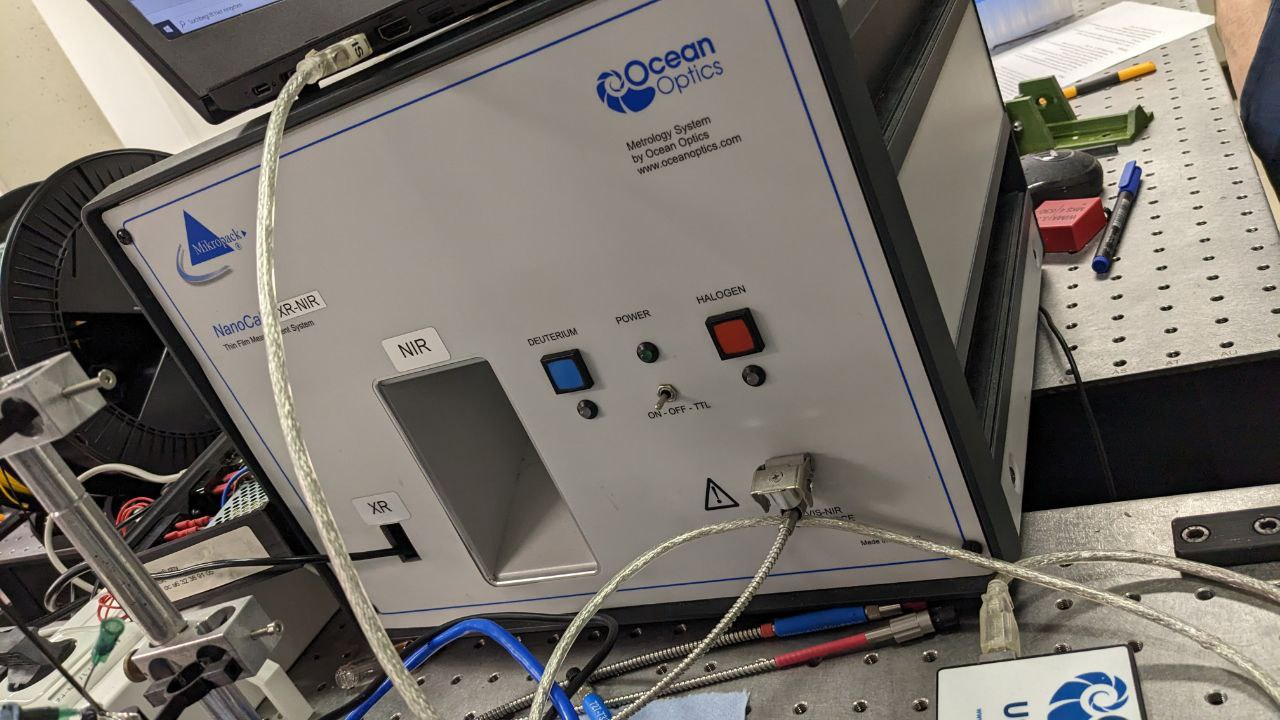
\includegraphics[scale = 0.15]{Lichtquelle-vorne.jpg} & 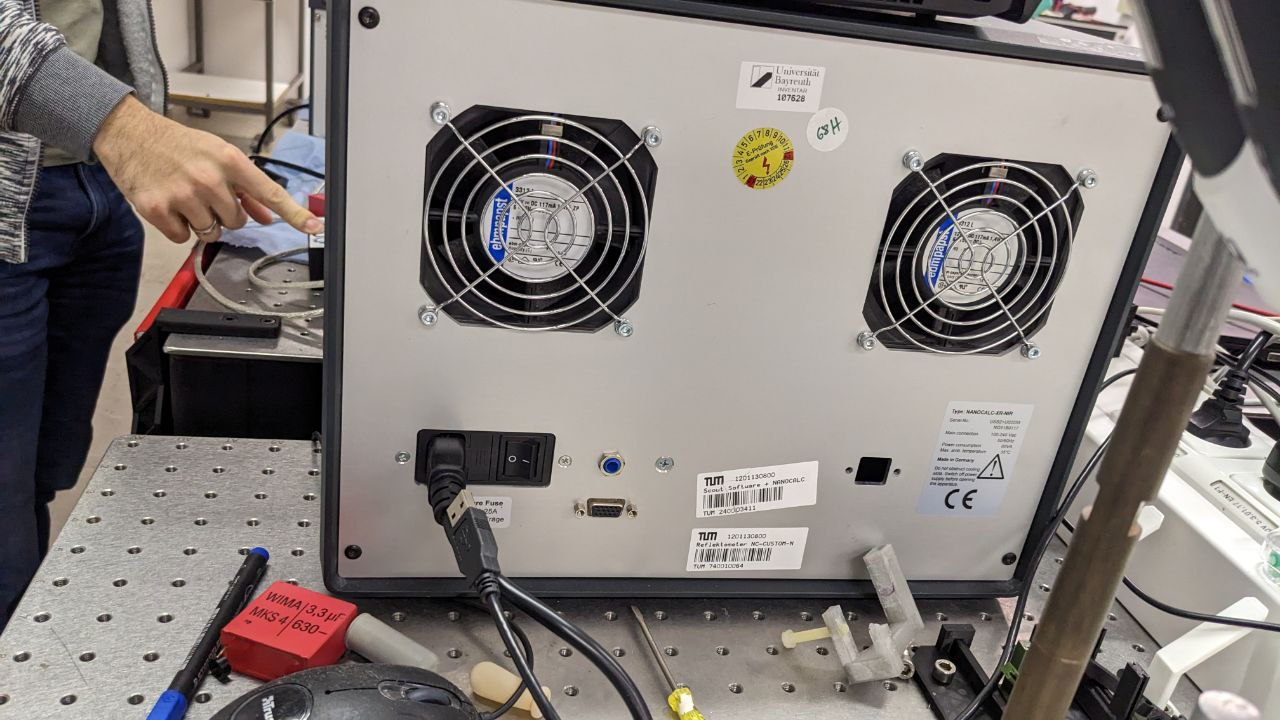
\includegraphics[scale = 0.15]{Lichtquelle-hinten.jpg}
	\end{tabular}
	\captionof{figure}{Halogen-Deuterium-Lampe (links Vorderansicht, rechts Hinteransicht)}
	\label{fig:lampe}
\end{center}
\newpage
Von der Halogen-Deuterium-Lampe gehen Glasfaserkabel zum Aufbau für die Reflexions und Transmissionsmessung [Abb. \ref{fig:mess}].
\begin{center}
	\captionsetup{type=figure}
	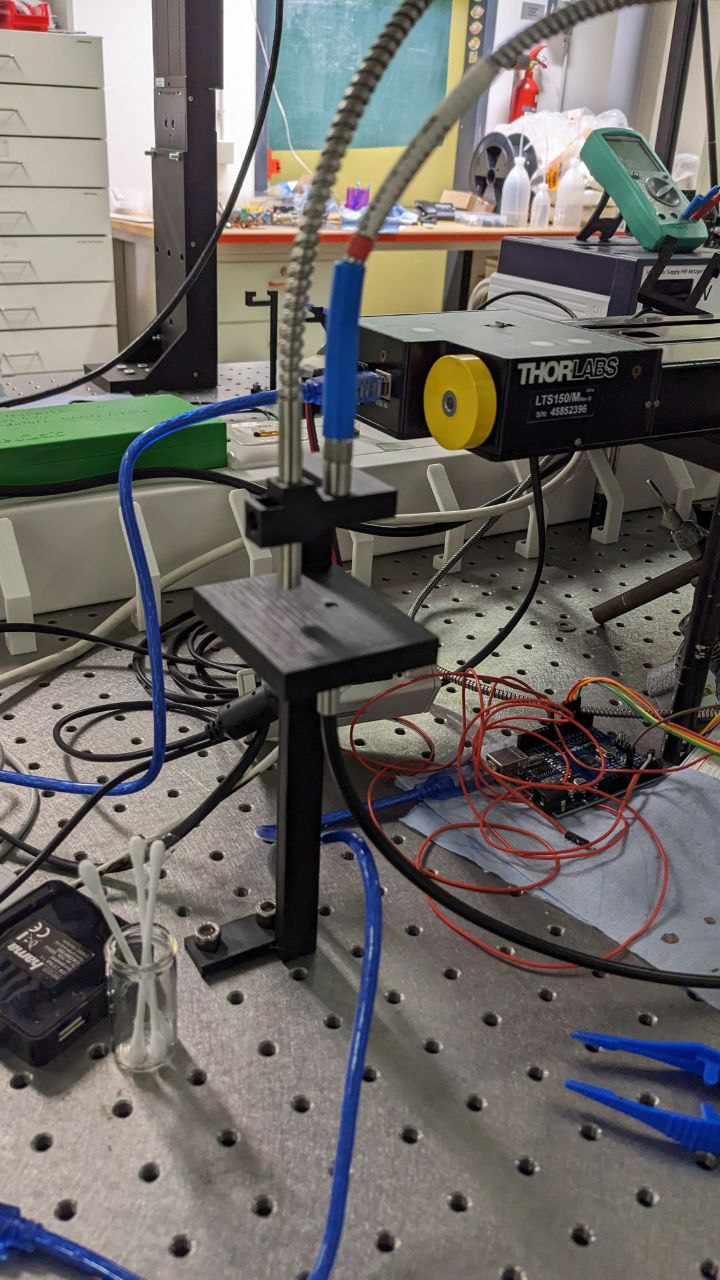
\includegraphics[scale = 0.15]{Messaufbau.jpg}
	\captionof{figure}{Messaufbau (links Reflexion, rechts Transmission)}
	\label{fig:mess}
\end{center}
Das Signal wird wiederum wieder von eine \textit{OceanOptics} Schnittstelle [Abb. \ref{fig:schnitt}] an den PC gesendet und von dem Messprogramm \textit{NanoCalc} ausgewertet.
\begin{center}
	\captionsetup{type=figure}
	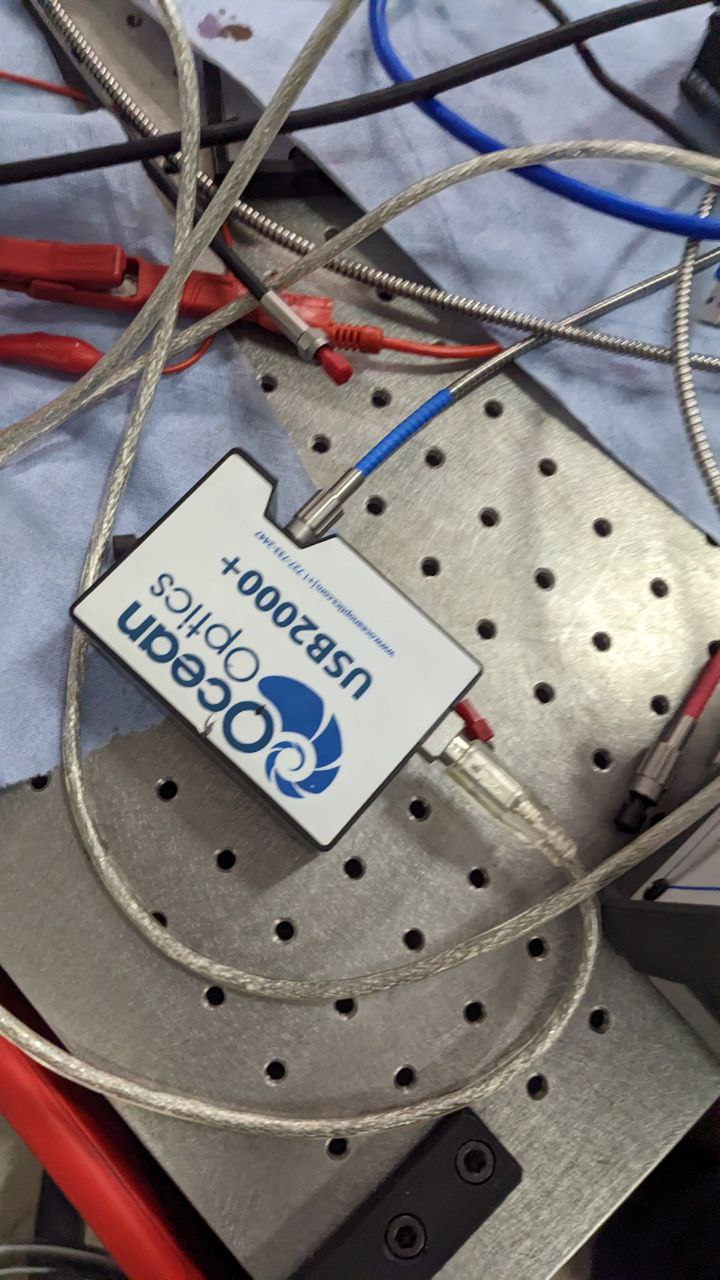
\includegraphics[scale = 0.15]{Schnittstelle.jpg}
	\captionof{figure}{Mikrocontroller zum verarbeiten des Signals}
	\label{fig:schnitt}
\end{center}
\newpage
Für alle Messungen wird die Probe \textit{19} als Referenzprobe genommen. Die Proben mit unterschiedlicher Konzentration werden 6 mal gemessen an 6 verschiedenen auf der Probe.\bigskip

Die Daten werden nach dem Schema:\\
\textit{(Konzentration)mg\_ml\_(Messungsnummer).xy}\\
und später in csv Dateien umgewandelt und umbenannt nach dem Schema:
\begin{itemize}
	\item \textit{Reflexion\_(Konzentration)mg\_ml\_(Messungsnummer).csv}
	\item \textit{Transmission\_(Konzentration)mg\_ml\_(Messungsnummer).csv}
\end{itemize}

Das Programm \textit{NanoCalc} fittet auch sofort für die gemessenen Werte die Dicke $d$ mit einem Parameter names Fitness, was eine Güte für den Fit ist. Die jeweiligen werte wurden in:
\begin{itemize}
	\item \textit{Reflexion\_(Konzentration)mg\_ml\_Fit.csv}
	\item \textit{Transmission\_(Konzentration)mg\_ml\_Fit.csv}
\end{itemize}
gespeichert. Dabei ist zu erwähnen, dass das Programm für die Konzentration von \SI{1}{\milli\gram\per\milli\litre} keinen Fit mehr machen konnte. \bigskip

Weiterhin wurden die Integrationszeit, boxcar und die Anzahl der Messung bevor gemittelt (Sample) wird für jede Messart geändert, welche in Tabelle \ref{tab:messPara} gegeben sind.
\begin{center}
	\captionsetup{type=table}
	\begin{tabular}{l | c c c}
		             & Integrationszeit in \si{\milli\sec} & boxcar in pixel & Sample \\
		\hline
		Reflexion    & 25								   & 1				 & 150    \\
		Transmission & 7								   & 1 				 & 600    
	\end{tabular}
	\caption{Veränderte Parameter in \textit{NanoCalc}}
	\label{tab:messPara}
\end{center} 